\section{Argument Schemes for Goal Modeling}
\label{sect:gmas}

\begin{table*}[h]
\centering
\begin{tabularx}{\textwidth}{|l|l|l|X|l|l|}
\hline
\multicolumn{2}{|c|}{\textbf{Argument scheme}} & \multicolumn{2}{c|}{\textbf{Critical Questions}} & \textbf{Effect}\\
\hline
AS0 & Actor $a$ is relevant & CQ0 &Is the actor relevant? & DISABLE\\
\hline
AS1 & Actor $a$ has resource $R$ & CQ1 &Is the resource available? & DISABLE\\
\hline
AS2 & Actor $a$ can perform task $T$ & CQ2 &Is the task possible? & DISABLE\\
\hline
AS3 & Actor $a$ has goal $G$ & CQ3 & Can the desired goal be realized? & DISABLE\\
\hline
AS4 & Actor $a$ has softgoal $S$ & CQ4 & Is the softgoal a legitimate softgoal?& DISABLE\\
\hline
\hline
AS5 & Goal $G$ decomposes into tasks $T_1,\ldots,T_n$ & CQ5a & Does the goal decompose into the tasks?& DISABLE\\
& & CQ5b & Does the goal decompose into any other tasks?& REPLACE\\
\hline
AS6 & Task $T$ contributes to softgoal $S$& CQ6a & Does the task contribute to the softgoal?& DISABLE\\
&& CQ6b & Are there alternative ways of contributing to the same softgoal?& INTRO \\
&& CQ6c & Does the task have a side effect which contribute negatively to some other softgoal?& INTRO\\
&& CQ6d & Does the task contribute to some other softgoal?& INTRO\\
\hline
AS7 & Goal $G$ contributes to softgoal $S$ & CQ7a & Does the goal contribute to the softgoal?& DISABLE\\
&& CQ7b & Does the goal contribute to some other softgoal?& INTRO\\
\hline
AS8 & Resource $R$ contributes to task $T$ & CQ8 & Is the resource required in order to perform the task?& DISABLE\\
\hline
AS9 & Actor $a$ depends on actor $b$ & CQ9 & Does the actor depend on any actors?& INTRO\\
\hline
AS10 & Task $T_1$ decomposes into tasks $T_2,\ldots,T_n$ & CQ10a & Does the task decompose into other tasks?& REPLACE\\
 &  & CQ10b & Is the decomposition type correct? (AND/OR/XOR)& REPLACE\\
\hline
AS11 & Task $T$ contributes negatively to softgoal $S$& CQ11 & Does the task contribute negatively to the softgoal?& DISABLE\\
\hline
\hline
AS12 & Element $IE$ is relevant & CQ12 & Is the element relevant/useful? & DISABLE\\
\hline
AS13 & Element $IE$ has name $n$ & CQ13 & Is the name clear/unambiguous? & REPLACE\\
\hline
\hline
- & - & Att & Generic counterargument & ATTACK\\
\hline
\end{tabularx}
\caption{List of argument schemes (AS0-AS13, left column), critical questions (CQ0-CQ12, middle column), and the effect of answering them (right column).}
\label{table:argument-schemes}
\end{table*}

In the previous section, we provided an overview of RationalGRL methodology. In this section, we discuss our argument schemes and critical questions in more detail. It is important to note that the list of argument schemes we present in this section is not exhaustive. It is an initial list that we have obtained by annotating transcripts, but our framework is fully extensible, meaning that new argument schemes and critical questions can be added depending on the problem domain.

The list of argument schemes and critical questions that we have obtained from our analysis is shown in Table~\ref{table:argument-schemes}. The first four argument schemes (AS0-AS4) are arguments for an element of a goal model, the next seven (AS5-AS11) are related to relationships, the next two (AS12-AS13) are for intentional elements in general, and the last is (Att) is a generic counterargument for any type of argument that has been put forward.

As we have already discussed in Section~\ref{sect:overview}, answering critical questions can have different impacts on the model. The right column in Table~\ref{table:argument-schemes} shows the impact of answering each critical question affirmatively. %SG: what does affirmatively mean?
As mentioned earlier, answering a critical question can create an argument disabling the corresponding GRL element of the attacked argument scheme (\textsf{DISABLE}); it can create an argument introducing a new GRL element (\textsf{INTRO}); it can replace the GRL element corresponding to the original argument (\textsf{REPLACE}), or it can simply attack an argument directly (\textsf{ATTACK}).

The RationalGRL language is an extension of GRL. The prototype tool we developed therefore also contains various new elements and a new relationship. The legend of the these additions is shown in Figure~\ref{fig:rationalgrllegend}.

In the following subsections, we first explain the new visual language in more detail, after which we provide details of the transcript annotation process with concrete examples (see Appendix~\ref{sect:transcripts:excerpts} for transcript excerpts).

\subsection{RationalGRL Language}

RationalGRL is an extension of GRL, and adds the following new elements (Figure~\ref{fig:rationalgrllegend}):
\begin{itemize}
\item \emph{Argument}: This represents an argument created by answering one of the critical questions which disables a GRL element, or counter-attacks a previous argument.
\item \emph{Disabled GRL element}: If a GRL element is attacked by an argument, which itself is not attacked, then this GRL element will be disabled, meaning that it does not play a role in the analysis of the GRL model. 
\item \emph{Refined GRL Element}: Not all critical questions attack a GRL element. It is also possible that a critical question \emph{replaces} an existing element (for instance, by clarifying the name of the element), or that it leads to the \emph{introduction} of a new element. In these cases, the corresponding GRL element is shown with a striped background. If the user clicks on this element, a details pane shows up containing the history of refinements (see Section~\ref{sect:tool}).
\item \emph{Attack Link}: An attack link can occur between an argument and a GRL element, or between two elements. It means that the source argument attacks the target GRL element or argument.
\end{itemize}

\begin{figure}[h]
\centering
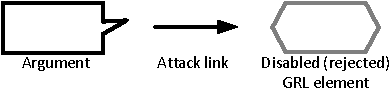
\includegraphics[width=0.35\textwidth]{img/legend}
\caption{The new elements and link of RationalGRL}
\label{fig:rationalgrllegend}
\end{figure}

\subsection{Details experiment}

The transcripts we used are created as part of two master theses on improving design reasoning~\cite{masterthesis1,masterthesis2}.

\paragraph{Subjects} The subjects for the case study are three teams of Master students from the University of Utrecht, following a Software Architecture course. Two teams consist of three students, and one team consists of two students.

\paragraph{Experimental Setup} The goal of the experiment is to design a traffic simulator. Participants were asked to use a think-aloud method during the design session. The assignment was slightly adjusted to include several viewpoints as an end product in order to conform to the course material~\cite{Bass:2012:SAP:2392670}. The full problem descriptions can be found in Appendix~\ref{sect:designprompt}. All groups were instructed to apply the \emph{functional architecture method}, focusing on developing the \emph{context}, the \emph{functional}, and the \emph{informational} viewpoints of the traffic simulator software. The students had two hours for the tasks. The entire discussion was documented in transcripts. The details of the transcripts are shown in Table~\ref{table:transcripts:info}.

\begin{table}[ht]
\centering
\begin{tabular}{|l|l|l|l|}
\hline
& transcript $t_1$ & transcript $t_2$ & transcript $t_3$\\
\hline
participants & 2 & 3 & 3\\
\hline
duration & 1h34m52s & 1h13m39s & 1h17m20s\\
\hline
\end{tabular}
\caption{Number of participants and duration of the transcripts.}
\label{table:transcripts:info}
\end{table}

\paragraph{Process of Extracting Argument Schemes and Critical Questions} %TODO I changed the title from annotation method. %MvZ: ok, looks good.

To develop the list of argument schemes and critical questions, we started with an initial list of 8 argument schemes and 18 critical questions that we derived from PRAS (AS1-AS4, AS6-AS9 of Table~\ref{table:argument-schemes}). We, then, annotated transcripts with arguments and critical questions from this initial list. If there were arguments or critical questions that did not appear in the initial list, we added them to the list.
% Existing argument schemes that did not appear were removed from the list, but critical questions were not removed (see discussion in Section~\ref{sect:gmas:transcripts:analysis}). 
%TODO I don't understand it! why?
%MvZ: I agree it is confusing. The idea is that critical questions are often implicit, so we kept them in since we believe it may still stimulate discussions. I now simply left it out since it doesn't add much and will only be confusing.

Most of the occurrences were not literally found back, but had to be inferred from the context. This can be seen in the various examples we will discuss.

%It is generally known in the argumentation literature that it can be very difficult to identify arguments in natural language texts~\cite{walton-etal2004}. Arguments are often imprecise, lack conclusion, and may be supported by nonverbal communication that is not captured in transcripts. However, there is hardly any research on argument extraction in the requirement engineering domain. Thus, despite this potential weakness in our approach, we believe it nevertheless is at least useful as something that others can build further on (see Section~\ref{sect:goalmodeling:openissues}). 
%TODO I don't understand the last few sentences... what does argument extraction mean? why is it needed? don't use "something that others" it is very informal for a journal paper. 
%MvZ: I was also sceptical about this paragraph when I wrote it. I think it belongs in the related work section where we can discuss it in more detail. I now removed it here.

\subsection{Experiment Results}

\begin{figure*}[h!]
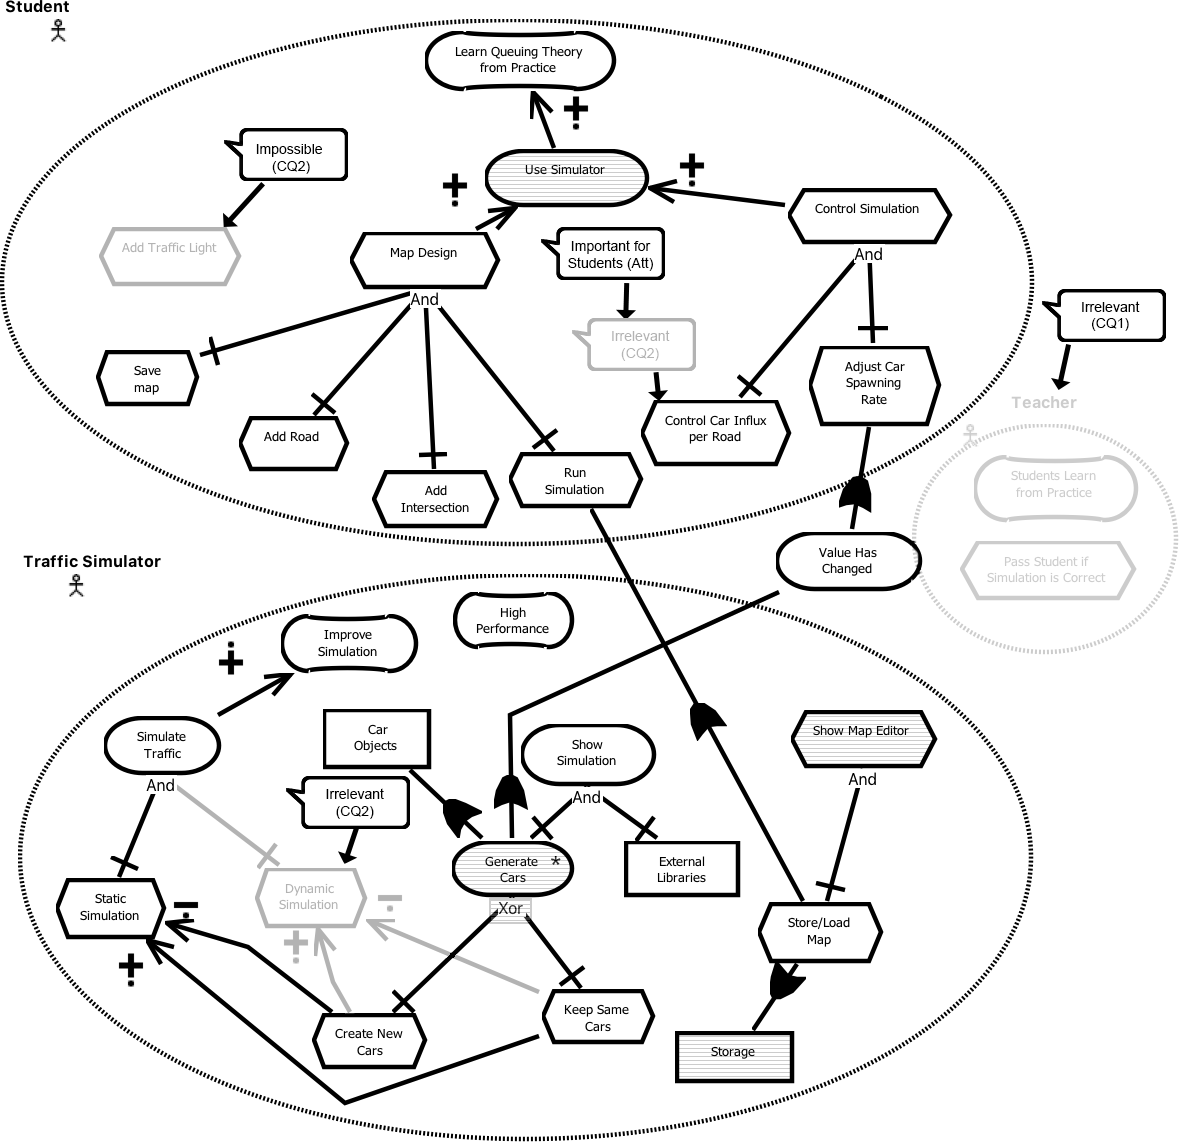
\includegraphics[width=\textwidth]{img/Fig6}
\caption{The GRL model manually constructed from transcript $t_1$. Green dots indicate accepted underlying arguments, red dots indicate rejected underlying arguments. Elements and relationships with no dot have been inferred by us.}
\label{fig:transcripts:grl}
\end{figure*} %TODO Figure doesn't match the text!

All original transcripts, annotations, and models are available on the following website \todo{Marc}{Marc}{Change URL and put everything together with the tool}:
\begin{quote} \url{http://www.github.com/marcvanzee/RationalArchitecture}
\end{quote}
We also provide excerpts of the annotation in Appendix~\ref{sect:transcripts:excerpts}, and most of the examples we use in this article come from the transcripts.

We found a total of 159 instantiation of argument schemes AS0-AS11 in transcripts. The most used argument scheme was AS2: ``Actor $A$ has task $T$'', however, each argument scheme is found in transcripts at least twice (Table~\ref{table:transcripts:results:argumentschemes}). A large portion (about 60\%) of argument schemes involved discussions about tasks of the information system (AS2, AS10).

We annotated 41 applications of critical questions. Many critical questions (about 55\%) involved clarifying the name of an element, or discussing its relevance (CQ12, CQ13).

\begin{table}[ht]
\centering
\begin{tabularx}{0.5\textwidth}{|l|X|l|l|l|>{\bfseries}l|}
\hline
\multicolumn{2}{|c|}{\textbf{Scheme/Question}} & $t_1$ & $t_2$ & $t_3$ & \textbf{total}\\
\hline 
AS0 & Actor & 2 & 2 & 5 & 9\\
\hline
AS1 & Resource & 2 & 4 & 5 & 11\\
\hline
AS2 & Task/action & 20 & 21 & 17 & 58\\
\hline
AS3 & Goal & 0 & 2 & 2 & 4\\
\hline
AS4 & Softgoal & 3 & 4 & 2 & 9\\
\hline
AS5 & Goal decomposes into tasks & 4 &0& 4 & 8\\
\hline
AS6 & Task contributes to softgoal & 6 & 2 &0& 8\\
\hline
AS7 & Goal contributes to softgoal &0& 1 & 1 & 2\\
\hline
AS8 & Resource contributes to task & 0 & 4 & 3 & 7\\
\hline
AS9 & Actor depends on actor &0& 1 & 3 & 4\\
\hline
AS10 & Task decomposes into tasks & 11 &14 &11 &36\\ 
\hline
AS11 & Task contributes negatively to softgoal & 2 & 1 & 0 & 3\\
\hline
\hline
CQ2 & Task is possible? & 2 & 2 & 1 & 5\\
\hline		
CQ5a & Does the goal decompose into the tasks? & 0 & 1 & 0 & 1\\
\hline
CQ5b & Goes decomposes into other tasks? & 1 & 0 & 0 & 1\\
\hline
CQ6b & Task has negative side effects? & 2 & 0 & 0 & 2\\
\hline
CQ10a & Task decompose into other tasks? & 1 &2 &0&3\\
\hline
CQ10b & Decomposition type correct? &1 &0& 1 &2\\
\hline
\hline
CQ12 & Is the element relevant/useful? & 2 & 3 & 2 &7\\
\hline
CQ13 & Is the name clear/unambiguous? &3 &10 & 3 & 16\\
\hline
\hline
- & Generic counterargument & 0& 2 & 2 & 4\\
\hline
\hline
\multicolumn{2}{|c|}{\textbf{TOTAL}}&69&80&69&222\\
\hline
\end{tabularx}
\caption{Number of occurrences of AS0-AS9, CQ0-CQ12 in the transcripts. Critical questions not appearing in this table were not found back in the transcripts.}
\label{table:transcripts:results:argumentschemes}
\end{table}

We manually created RationalGRL models from argument schemes and critical questions found in each transcript, to verify whether the arguments put forward by the participants were sufficiently informative. An example of such a model is shown in Figure~\ref{fig:transcripts:grl}. This figure shows a simplified version of the actual model in order to improve the presentation, but the full models can be found back in our repository. \todo{Marc}{all}{Perhaps we should explain a bit about the model here?}

Answering a critical question can have four different effects on the original argument and the corresponding GRL element:
\begin{itemize} 
\item \textsf{INTRO}: Introduce a new goal element or relationship with a corresponding argument. This operation does not attack the original argument of the critical question, but rather creates a new argument. In Figure~\ref{fig:transcripts:grl}, each GRL element can be seen as the instantiation of an argument scheme. For instance, the XOR-decomposition from ``Generate Cars'' is an instantiation of AS5 as follows: ``Goal \texttt{Generate cars} XOR-decomposes into tasks \texttt{Keep same cars} and \texttt{Create new cars}''. Suppose now that the modelers that created Figure~\ref{fig:transcripts:grl} would continue their analysis by discussing critical question CQ5b: ``Does the goal \texttt{Generate cars} decompose into other tasks?'', and that they would answer this with ``Yes, namely \texttt{Choose randomly}''. This then results in the introduction of another task with the name ``Choose randomly'', and the XOR-decomposes would go from ``Generate Cars'' into the three tasks \texttt{Keep same cars}, \texttt{Create new cars}, and \texttt{Choose randomly}.''
\item \textsf{DISABLE:} Disable the element or relationship of argument scheme to which critical questions pertains. This operation does not create a new argument, but it only disables (i.e., attacks) the original one. In Figure~\ref{fig:transcripts:grl}, there are several examples of disabled GRL elements. The task ``Add traffic light'' (top-left in figure) is attacked by answering critical question CQ2: ``Is task Add traffic light possible?'' negatively, resulting in an argument that disables the GRL element. What we also see from Figure~\ref{fig:transcripts:grl} is that disabling actor ``Teacher'' also disables all elements belonging to this actor. Furthermore, disabling task ``Dynamic simulation'' also disables all incoming and outgoing links with this task.

\item \textsf{REPLACE:} Replace the element of the argument scheme with a new element. In Figure~\ref{fig:transcripts:grl}, task ``Show map editor'' has been replaced various times, and this is shown in the figure as a \emph{refined} element. In this case, the participants were discussing the correct naming for this element (CQ13), leading to various replacements of the name. While the previous names are not shown in the figure, they show up in the details pane of the corresponding element.
\item \textsf{ATTACK:} Attack any argument with an argument that cannot be classified as a critical question. In Figure~\ref{fig:transcripts:grl} we see one example of such a counter-attack. First, task ``Control car influx per road'' is attack by answering CQ2 (irrelevant task). However, after discussing this, the participants found that this was not the case, since the problem description stated that it is important that students can control the simulation manually. Therefore, the arguments that attacked the task is attacked by the counter-argument ``Important for students'', which re-enables the task ``Control car influx per road''. We provide a precise semantics for this in Figure~\ref{sect:formalframework}.
\end{itemize}

%MvZ: I completely removed the subsection below. I think it doesn't add much and it is confusing. What do you think?

%\subsection{Analysis}
%\label{sect:gmas:transcripts:analysis}

%\paragraph{Analysis of Argument Schemes}
%Recall that our initial list of argument schemes consists of AS1-AS4, AS6-AS9 (Table~\ref{table:argument-schemes}). Therefore, the difference between the initial list of argument schemes and those found in transcripts is quite small. 
%TODO The next few sentences are weird... they make our work very trivial.. rewrite.
%We found it surprising that we were able to find back all the schemes in the transcript at least twice, even more since the topic of discussion was not goal models, but more generally the architecture of an information system. This gives us an indication that it is possible to capture (parts of the) arguments used in those type of discussions using argument schemes.

%We observed that our initial list is rather limited, which is a consequence of the fact that it is derived from PRAS. Since PRAS only considers very specific types of relationships, we are not able to capture many other relationships existing in GRL. GRL has four types of intentional elements (softgoal, goal, task, resource) and four types of relationships (positive contribution, negative contribution\footnote{In fact, a contribution can be any integer in the domain [-100,100], but for the sake of simplicity we only consider two kinds of contributions here.}, dependency, decomposition), allowing theoretically $4^3=64$ different types of argument schemes, of which we currently only consider 11. 
%TODO which analysis? why aren't they used? How did we empirically validate it? How are we confident in the result?
%Our analysis, however, shows that many of these schemes are not often used, and thus, gives us some confidence in the resulting list. However, additional argument schemes and critical questions can be easily added to our framework. Beside, our list is not meant to be exhaustive.

%\paragraph{Analysis of the Critical Questions} The difference between the initial list of critical questions and those we found in transcripts is much larger than for the critical questions. %TODO  I don't get this sentence. Also, the ones below. 
%We found few of the critical questions we initially proposed. %TODO ???
%However, this does not mean that they were not implicitly used in the minds of the participants. If a participant, for instance, forms an argument for a contribution from a task to a softgoal, it may very well be that she/he was asking her/him-self the question ``Does the task contributes to some other softgoals?''. However, many of these critical questions are not mentioned explicitly. If we assume this explanation is at least partially correct, then this would mean that critical questions may still play a role when formalizing the discussions leading up to a goal model, and it would be limiting to leave them out of our framework. In the context of a tool support, we believe that having these critical questions available may stimulate discussions. %TODO what does it mean in the context of a tool support?